\label{microSD}

Zunächst sollten die gemessenen CO$_2$-Werte auf dem Arduino selbst abgespeichert werden. Der EEPROM wäre dafür die Lösung gewesen. Jedoch besitzt dieser eine Speicherkapazität von 1KB. Bei größeren Messungen reicht das unter Umständen nicht aus, sodass eine Methode gefunden werden musste, in welcher die Daten extern vom Arduino abgespeichert werden können. \\
Dazu haben wir den, in Abbildung \ref{fig:SD-Modul} zu sehenden Mikro-SD-Karten-Adapter hinzugezogen. Hier können die gemessenen CO$_2$-Werte ohne Speicherprobleme gesichert werden. \\

\begin{figure}[!hbt]
	\centering
	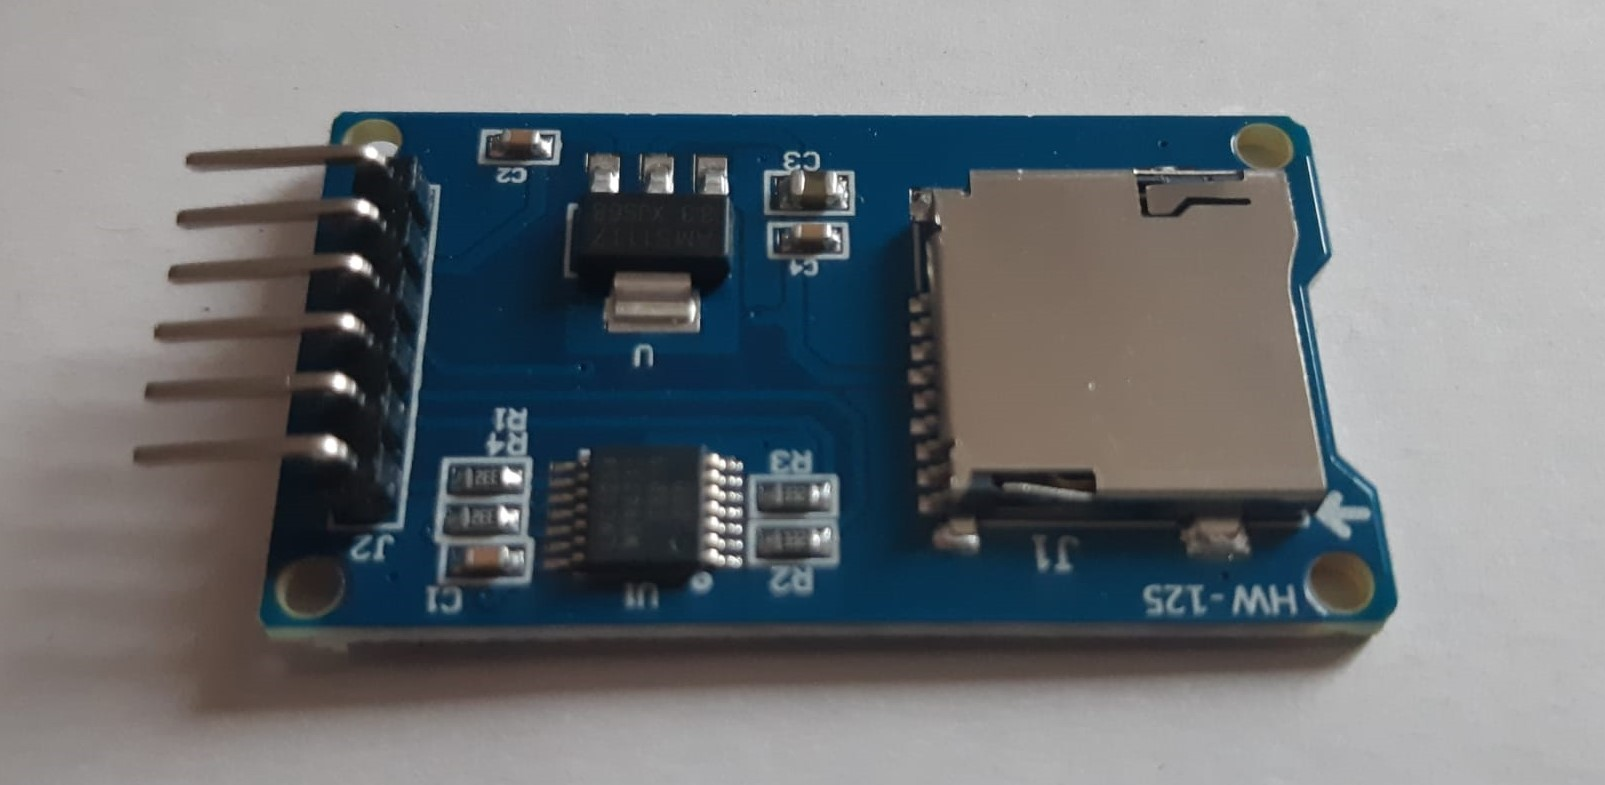
\includegraphics[width=0.7\linewidth]{Images/Mikro-SD_2}
	\footnotesize{\\ Quelle: eigene Aufnahme}
	\caption{Verwendeter Mikro-SD-Karten-Adapter, mit Sicht auf dessen Vorderseite}
	\label{fig:SD-Modul}
\end{figure}

Der Mikro-SD-Karten-Adapter ist über die, in Abbildung \ref{fig:SD-Modul_RUCK} zu sehenden PINs MISO, MOSI, SCK und CS, mit dem Arduino verbunden. Die komplementären PINs des Arduinos sind in Abbildung \ref{fig:Layout} zu sehen. Der Adapter benötigt zudem eine Versorgungsspannung von mindestens $4,5\volt$ bis maximal $5,5\volt$ zur Masse. \cite[vgl. S. 1]{ebaySearch.} \\

\begin{figure}[!hbt]
	\centering
	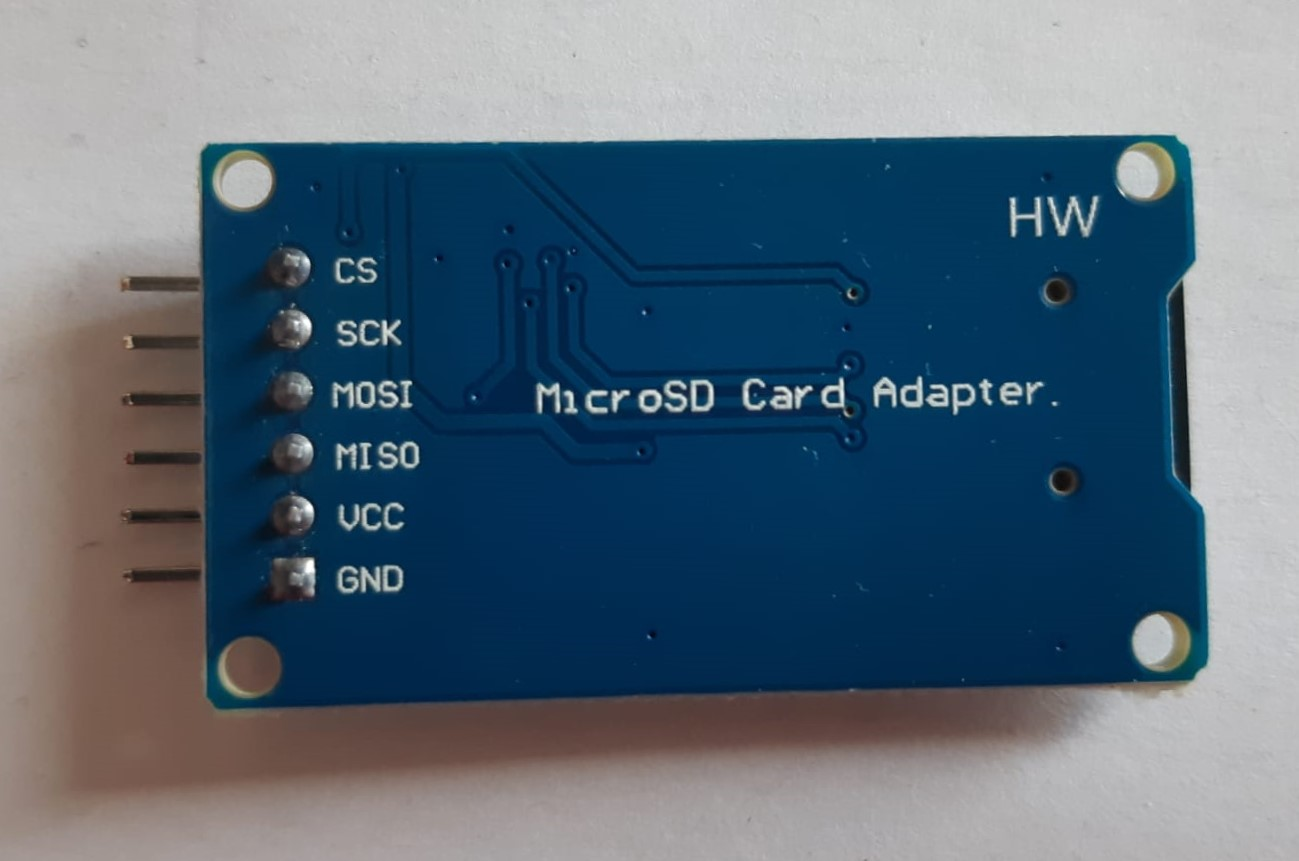
\includegraphics[width=0.6\linewidth]{Images/Mikro-SD_3}
	\footnotesize{\\ Quelle: eigene Aufnahme}
	\caption{Verwendeter Mikro-SD-Karten-Adapter, mit Sicht auf dessen Rückseite}
	\label{fig:SD-Modul_RUCK}
\end{figure}

Für die Integration der SD-Karte, muss zunächst die Bibliothek <SD.h> eingebunden werden. Anschließend wird eine globale Variable als File deklariert. In unserem Programmablauf wird die anschließende Initialisierung der SD-Karte zweimal durchgeführt. Das erste mal im Setup, vor dem Programmablauf. Die Begründung liegt darin, dass dem Benutzer bei fehlender SD-Karte schon vor der Auswahl des Messmodus eine Fehlermeldung angezeigt werden kann. Das zweite Mal wird die SD-Karte vor dem Start der Messung durchgeführt. Das hat den Hintergrund, dass die SD-Karte kurz davor entfernt werden könnte. Auch hier wird bei fehlender Karte der Benutzer durch eine Ausgabe informiert. Zudem wird das Programm anschließend neu gestartet. \\
Vor dem Start der Messung wird außerdem eine .txt-Datei auf der SD-Karte erstellt. Im Fall, dass eine gleichnamige Textdatei bereits existiert, wird diese zum schreiben geöffnet. An dieser Stelle wird im Programmcode auch definiert, dass der Arduino die SD-Karte beschreiben und nicht auslesen soll. \\
Während der Messung bleibt die SD-Karte geöffnet und der Arduino im Schreibe-Modus, sodass kein lokaler Speicher für die Übertragung der Daten benötigt wird. Somit können so viele Messungen durchgeführt werden, wie Speicherkapazität auf der SD-Karte vorhanden ist. Nach Beenden der Messung wird die Textdatei abgespeichert und geschlossen. \\

\begin{figure}[!hbt]
	\centering
	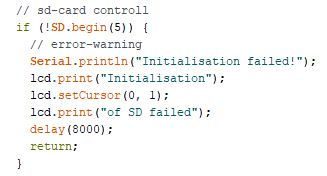
\includegraphics[width=0.6\linewidth]{Images/sdSetup}
	\footnotesize{\\ Quelle: eigene Aufnahme}
	\caption{Codeausschnitt zur Initialisierung der SD-Karte im Setup aus dem Quellcode}
	\label{fig:SD_Setup}
\end{figure}

